
\section{Boyer-Moore}

\subsection{Intro to Boyer Moore}
The key components in the Boyer-Moore algorithm are the right-to-left scan, the Bad Character Rule and the Good Suffix rule, which play a crucial role in improving the search process, as they are methods used to determine the amount by which a pattern can be shifted to the right during a search. By utilising the Good suffix rule and the Bad Character Rule, the algorithm reduces the number of unnecessary comparisons and skips larger portions of the search text. This allows the algorithm to avoid reading the entire text and in the best case achieve a sub-linear running time of $\Omega(m/n)$, thus performing better than KMP in the best case. The Boyer-Moore algorithm runs in $O(m)$ time when the pattern does not appear in the text and in general $O(n\cdot m)$ when the pattern does appear. The case where one is only interested in finding the first occurrence of a pattern is the same as when the pattern does not appear in the text: $O(m)$. Additionally, the Apostolico-Giancarlo extension of the algorithm makes it a $O(m)$ time in all cases. 

\subsection{Right to left scan}
In contrast to the naive methods, which use a left-to-right scan, the Boyer-Moore algorithm uses a right-to-left scan. Firstly the pattern is placed such that the first character of the pattern aligns with the first character of the search text. The first characters that are compared are however the right-most character of the pattern and the aligned letter of the text. \kommentar{eksempel på hvordan det giver best-case m/n} If it is a match it continues to compare the characters to the left.

\subsection{The Bad Character Rule}
There exists an Extended Bad Character Rule besides the Bad Character Rule. The original Boyer-Moore Algorithm only used the Bad Character Rule. This chapter will introduce both of them and in section \ref{sec:goodsuffixvsbadcharacter} it will be proven that the Extended Bad Character rule is obsolete when combined with the Good Suffix Rule. The Extended Bad Character rule can however have a use case on its own when the Good Suffix rule is not involved. 

\subsubsection{The Bad Character Rule}
When a mismatch occurs between a character $c_p$ from the pattern and a character $c_t$ from the text, the Bad Character Rule reasons that the pattern can be shifted, so that the rightmost occurrence of $c_t$ in the pattern matches $c_t$ in the text, if the occurrence is placed to the left of the mismatch. If the rightmost occurrence is placed on the right of the mismatch, the Bad Character Rule can only shift the pattern once. If no occurrences of $c_t$ exist in the pattern then the patterns can be shifted to the left until there no longer is an overlap of the pattern and $c_t$.

\subsubsection{The Extended Bad Character Rule}
Extended Bad Character Rule is the addition that not only the right-most occurrence of a character is kept, but all occurrences, so the pattern can be shifted until the next time the character $c_t$ occurs. If the mismatch happens at the most left character of the pattern, the Bad Character Rule only allows shifting the pattern one step further.  If no occurrences of $c_t$ exist in the pattern then the patterns can still be shifted to the left until there no longer is an overlap of the pattern and $c_t$. An example where the Bad Character rule is used along with the difference between the regular and extended rule is shown in figure \ref{fig:badcharacterrule_example}. 

\begin{figure}[t]
\begin{verbatim}
      0        1                  0        1             0        1      
      1234567890123456            12345678901            12345678901
   T: SomeBadCharacter         T: aabbabacdab         T: aabbabacdab
   P: BadCharacter             P: bacdab              P: bacdab          
                 *                   *^^                    *^^     
          BadCharacter             bacdab                   bacdab  
          ^^^^^^^^^^^^                                              
\end{verbatim}
\caption{Showing the bad character rule shifting successfully, the rule only shifting one position and the extended bad character rule being better in that case}
\label{fig:badcharacterrule_example}
\end{figure}

\subsubsection{R(x) values}
To calculate the number of characters the algorithm is allowed to skip, using the Bad Character Rule, without skipping the starting position of a potential match, the $R(x)$ values need to be introduced. 

\begin{itemize}
    \item[] \textbf{Definition} For each character in the alphabet, let $R(x)$ be the position of the rightmost occurrence of character $x$ in the pattern. $R(x)$ is defined to be zero if $x$ does not occur in $P$.
\end{itemize}

The $R(x)$ values can be calculated in $\Theta(n)$ time using a hash map. The hash map has a key for every letter in the pattern and each key has a value representing at which position the rightmost occurrence of the letter is at. By iterating through the pattern from right to left, the position of a character in the pattern can be saved in the hash map if the key representing that letter does not yet have a value. In this way, $R(x)$ is calculated in $\Theta(n)$ time and is only using linear extra space in the size of the number of unique letters in the pattern.

%\kommentar{Figure om R(x) non extended values}

When using the Extended Bad Character Rule, it is not only the rightmost occurrence of character, that is necessary to save the position of, but all occurrences. This is because the pattern may be shifted to the rightmost occurrence of the $c_t$ to the left of a mismatch. Now it is necessary to use $R_i(x)$ values.

\begin{itemize}
    \item[] \textbf{Definition} For each character in the alphabet, let $R_i(x)$ be the right-most occurrence of character $x$ in the pattern to the left of position $i$. $R_i(x)$ is defined to be zero if $x$ does not occur in $P$ to the left of position $i$.
\end{itemize}

A hash map can still be used to keep of these $R_i(x)$ values, but the values of each key are now a list of positions in descending order. The lists are generated by iterating through the pattern from left to right, adding all positions of characters to the representative list in the hash map. This still takes $\Theta(n)$ time but now also uses $\Theta(n)$ space, as the position of each character in the pattern is added to some list.

%\kommentar{Figure om R(x) extended values}

With these definitions of $R(x)$ and $R_i(x)$ values, the Bad Character Rule and Extended Bad Character Rule can now be formally defined:

\begin{itemize}
    \item[] \textbf{Bad Character Rule} When a mismatch occurs at position $i$ in $P$ with character $x$ in $T$, look up the $R(x)$ value. If $R(x)<i$, then shift the pattern $i-R(x)$ positions so that $P(R(x))$ matches the $x$ in $T$ or the pattern is shifted beyond the $x$ if $R(x)=0$. If $R(x)>i$, then shift by one position. 
    \item[] \textbf{Extended Bad Character Rule} When a mismatch occurs at position $i$ in $P$ with character $x$ in $T$, shift $P$ by $i-R_i(x)$ positions, so $P(R_i(x))$ matches the $x$ in $T$ if $R_i(x)>0$, or the pattern is shifted beyond the $x$ if $R_i(x)=0$. 
\end{itemize}

\subsection{The Good Suffix rule}

\begin{figure}[b!]
    \centering
    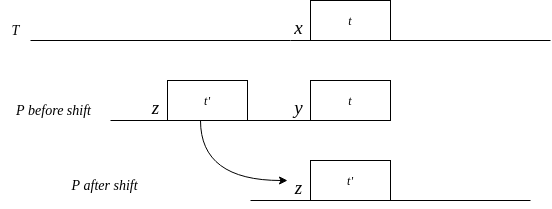
\includegraphics[width=\textwidth]{LaTeX/Figures/Zalg/suffixrule.png}
    \caption{Strong Good Suffix rule. The suffix $t$ matches but the next character mismatches $y\neq x$. Shift $P$ to the next time $t$ occurs with a different preceding character. }
    \label{fig:suffixrule}
\end{figure}

The Good Suffix rule is the other half of the Boyer-Moore algorithm and requires some more involved preprocessing. It is here that the Z algorithm can be used to more easily compute certain values and do so in linear time. There exist both a strong and a weak version of the Good Suffix rule, where the original Boyer-Moore only used the weak version\cite{Gusfield1997AlgorithmsOS}, but the strong version can make larger shifts with no added time or space. This section focuses on the strong version. 

\begin{itemize}
    \item[] \textbf{Strong Good Suffix Rule} When a suffix of $P$ has been matched with a substring $t$ of $T$ and a mismatch occurs at the next preceding character, then find in $P$ the right-most copy $t'$ of $t$ of in $P$ such that the character preceding $t'$ is different from the character preceding $t$ in $P$ ($z\neq y$ in figure \ref{fig:suffixrule}) and shift $P$ so that $t'$ in $P$ aligns with $t$ in $T$. If no such occurrence of $t'$ exists in $P$, shift $P$ by the least amount so that a prefix of $P$ aligns and matches a suffix of $t$ in $T$. If that is not possible, shift $P$ entirely past $t$ in $T$. 
    \item[] \textbf{Occurrence of P} When an occurrence of $P$ is found in $T$, shift $P$ by the least amount so that a prefix of $P$ aligns and matches a suffix of $P$ in $T$. If that is not possible, shift $P$ entirely past $P$ in $T$. 
\end{itemize}

In order to support this rule, $L'(i)$ and $l'(i)$ values are to be computed from $P$ in the preprocessing step. $L'(i)$ is used to find the occurrence of $t'$ in $P$ where $t=P[i..n]$, and $l'(i)$ is used to shift $P$ (by the least amount) so that a prefix of $P$ matches a suffix of $P[i..n]$. They are defined as follows:

\begin{itemize}
    \item[] \textbf{Definition} For each $i$, $L'(i)$ is the largest position less than $n$ such that the substring $P[i..n]$ matches a suffix of $P[1..L'(i)]$ and such that the character (if it exists) preceding that suffix is not equal to $P(i-1)$. $L'(i)$ is defined to be zero if there is no position satisfying the conditions. 
    \item[] \textbf{Definition} For each $i$, let $l'(i)$ denote the length of the longest suffix of $P[i..n]$ that is also a prefix of $P$. If none exists, $l'(i)$ is defined to be zero. 
\end{itemize}

Figure \ref{fig:gsr-example} shows the $N_j$, $L'$, and $l'$ values of the string \textit{tapftapgtapftap}.
% Her er et eksempel som kan flyttes til hvor det passer bedst. 
\begin{figure}[ht!]
\begin{verbatim}
                              0        1      
                              123456789012345 
                          S : tapftapgtapftap 
                          Nj: 00300070003000_ 
                          L': _00000007000b00 
                          l': _77777777333300 
\end{verbatim}
\caption{Example showing the values of $N_j$, $L'$, and $l'$ for the string $tapftapgtapftap$. The number $b$ means 11 and the symbol '$\_$' represents the value not being defined for that index. }
\label{fig:gsr-example}
\end{figure}

Using a theorem from \cite{Gusfield1997AlgorithmsOS} (Theorem 2.2.2), the Z algorithm can be used to compute the $L'(i)$ values in linear time. This simply extends to computing the $l'(i)$ values as well. It works as follows:

Use the Z algorithm on the reversed string $P^r$. These values can be used to compute new $N_j(P)$ values defined as $N_j(P)=Z_{n-j+1}(P^r)$. Since $Z_i(S)$ is the length of the longest substring of $S$ that starts at $i$ and matches a prefix of $S$, $N_j(P)$ corresponds to the length of the longest suffix of the substring $P[1..j]$ that is also a suffix of $P$. These values are, maybe unsurprising, very useful in finding the $L'(i)$ and $l'(i)$ values. 

Then it is clear that for each $i$, $L'(i)$ is the largest index $j$ less than $n$ such that $N_j(P)=|P[i..n]|=n-i+1$. Additionally, $l'(i)$ equals the largest $j\leq|P[i..n]|=n-i+1$ such that $N_j(P)=j$. 

Combining these results, the $L'(i)$ and $l'(i)$ values can be computed using the following algorithm:

\begin{algorithm}
\caption{Computing $L'(i)$ and $l'(i)$}\label{alg:Lvalues}
\begin{algorithmic}
\State Initialise $L'(i):=0$ and $l'(i):=0$ for all $i$. 
\For{$j=1..n-1$}
    \If{$N_j>0$}
        \State $i:=n-N_j+1$
        \State $L'(i):=j$
    \EndIf
\EndFor
\For{$j=1..n-1$}
    \If{$N_j=j$}
    \State $l'(n-j+1) := j$
    \Else
    \State $l'(n-j+1) := l'(n-j+2)$ \Comment{$l'(n+1)$ is defined to be $0$}
    \EndIf
\EndFor
\end{algorithmic}
\end{algorithm}

Finally, the Good Suffix rule can be defined more precisely using these values. 

\begin{itemize}
    \item[] \textbf{The Strong Good Suffix Rule with exact shifts} When a mismatch occurs at position $i-1$ of $P$, and $L'(i)>0$, then shift $P$ by $n-L'(i)$ positions. If $L'(i)=0$, meaning that $t'$ from figure \ref{fig:suffixrule} does not exist, shift the pattern by $n-l'(i)$ positions, which is the least amount so that a prefix of the shifted pattern matches a suffix of $t$. When an occurrence of $P$ is found, shift by $n-l'(2)$. These are correct even when $l'(i)=0$. In the case that the mismatch occurs at position $n$, then shift by only 1 position. 
\end{itemize}


\subsubsection{Interaction between the Good Suffix and the Extended Bad Character rule}\label{sec:goodsuffixvsbadcharacter}

As explained, the whole Boyer-Moore algorithm uses both the Bad Character rule and the Good Suffix rule to determine how far to shift the pattern without missing a possible occurrence in the text. An interesting nontrivial fact is that when using the Good Suffix rule, the Extended Bad Character rule will actually never be better than using just the Bad Character rule. More formally:

\begin{itemize}
    \item[] \textbf{Lemma 1} When a mismatch occurs in position $i$ of $P$ with a character $x$ in $T$ and $x$ occurs in $P$ to the right of position $i$, the Good Suffix rule will always shift $P$ more than the Extended Bad Character rule, making the Extended Bad Character Rule no better than the regular Bad Character rule. 
\end{itemize}

\begin{figure}[t]
    \centering
    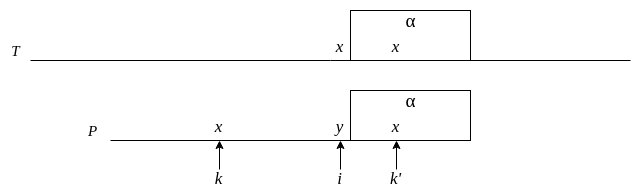
\includegraphics[width=\textwidth]{LaTeX/Figures/Zalg/suffixvsbadchar.png}
    \caption{The suffix $\alpha$ of $P$ matches with $T$ until mismatching character $x$ in $T$ at position with position $i$ in $P$. The next $x$ to the left of position $i$ occurs at position $k$ and the next $x$ to the right at position $k'$.}
    \label{fig:suffixvsbadchar}
\end{figure}

\subsubsection{Proof}

Let $\alpha=P[i+1..|P|]$ be the suffix of $P$ that has matched a substring of $T$ until the mismatch. Since it is assumed that $x$ occurs in $\alpha$, let $k'$ be the left-most position of such an $x$. Further, let $k$ be the position of the right-most $x$ in the prefix $P[1..i-1]$ - if no such $x$ exists, $k$ is defined to be zero. See figure \ref{fig:suffixvsbadchar}. 

Since the mismatching character occurs in $P$ to the right of the mismatch, the regular Bad Character Rule gives no information and could only shift $P$ by one position, so this is the only case where the extended rule would be used. The Extended Bad Character rule would shift $P$ to the right until the next occurrence of $x$ matches with the mismatched $x$ in $T$. Thus, the Extended Bad Character Rule will shift $P$ by $i-k$ positions, also when $k=0$. 

The Good Suffix Rule looks for an occurrence of $\alpha$ in $P$. First assume $k=0$. Then $\alpha$ does not occur again in $P$, and the Good Suffix rule will shift $P$ by $n-l'(i+1)$. In general, $l'(j)$ for any $j$ is at most $n-j+1$, but since $x$ does not occur in $P$ to the left of $k'$, then $l'(i+1)$ will be at most $n-k'$ and the Good Suffix rule will shift by at least $n-(n-k') = k'$ positions. 

If $k>0$, then either the substring $\alpha$ matches the $x$ in position $k'$ with the $x$ around position $k$, that is, at $S[k-(k'-i)+1\ ..\ k-(k'-i)+1+|\alpha|]$, or $\alpha$ matches at a position more to the left (or $\alpha$ does not match at all, shifting as mentioned above). This is because it is not possible for $\alpha$ to match a position where $k'$ would be shifted to the right of $k$ since, by construction, there is no occurrence of $x$ strictly between position $k$ and $k'$. This means the Suffix rule will shift by at least $k'-k$ in this case. 

Altogether, the Good Suffix rule will shift by at least $k'$ or $k'-k$ positions, both of which are larger shifts than $i-k$ from the Extended Bad Character rule. 

\rightline{$\square$}

\subsection{The whole Boyer-Moore algorithm}

The Boyer-Moore algorithm uses both the Bad Character rule and the Good Suffix rule to determine how far to shift the pattern when a mismatch occurs and since both rules ensure that they do not shift the pattern too far, it is best to shift by the maximum of the shifts given by the two rules. 

To summarise, the Boyer-Moore algorithm aligns the pattern with the text and uses a right-to-left scan to compare each character. When a mismatch occurs, the pattern is shifted to the right by an amount that is the maximum of what the Bad Character rule and the Good Suffix rule offers. When an occurrence of $P$ in $T$ is found, the pattern is shifted according to the Good Suffix rule. 

The best case for Boyer-Moore is when the right-most character of the pattern does not occur in the rest of the pattern and mismatches at every alignment of $P$ with $T$, resulting in an immediate shift of $n$ position. This results in a best-case time complexity of $\Omega(m/n)$. 

To analyse the run time of the algorithm, the worst-case example needs to be analysed. If the whole pattern is matched, it is shifted according to the Good Suffix Rule, which could be 1 position. The running time is hence $O(n\cdot m)$, as it in the worst case needs to match the whole pattern for each character of the text. An example of this worst case is when both the text and the pattern consist of the same repeated character, where Boyer-Moore becomes effectively identical to the Naive algorithm and makes exactly $n\cdot(m-n+1)$ comparisons. With the Apostolico-Giancarlo extension however, the algorithm matches and/or mismatches each character in the text at most once, resulting in at most $2m$ comparisons and giving $O(m)$ in all cases. 

\subsection{Apostolico-Giancarlo}

The problem with the Boyer-Moore algorithm is that it can match the same character in the text several times. For example, after matching a suffix of the pattern of length $|\alpha|$ and then shifting using the Good Suffix rule where $\alpha$ occurs again in the pattern, the Boyer-Moore algorithm forgets this and explicitly compares the characters again, see figure \ref{fig:apostolicoexample}. 

\begin{figure}[ht!]
\begin{verbatim}
                0        1                  0        1 
                12345678901                 12345678901
             T: abcbxyzxxyz              T: abcbxyzxxyz
             P: xyzxxyz                  P: xyzxxyz    
                   *^^^                        *^^^    
                    xyzxxyz                     xyzxxyz
                    ^^^^^^^                        ^^^^
\end{verbatim}
\caption{Example of a situation where the Boyer-Moore algorithm (left) matches three characters before shifting and then matches the whole pattern again. With the Apostolico-Giancarlo extension (right), the previously matched substring is not matched again. }
\label{fig:apostolicoexample}
\end{figure}

The Apostolico-Giancarlo extension uses a vector $M$ of length $m$ to remember how far a suffix of a previous alignment of $P$ has matched. During the algorithm, whenever the right end of the pattern is aligned with position $j$ in $T$, $M[j]$ will be assigned a value and $M[i]$ for other indices is undefined. The value assigned to $M[j]$ signals that a suffix of $P$ of length at least $M[j]$ matches the text ending in position $j$. 

Recall that for a string $P$, the value $N_i(P)$ is the length of the longest suffix of $P[1..i]$ that matches a suffix of $P$. In this extension, this value is compared to a corresponding value in $M$ to speed up the Boyer-Moore algorithm. As an example, suppose that $P$ has matched $T$ up to position $i$ which is aligned with position $h$ in $T$ and that $M[h]>N_i$, see figure \ref{fig:Apostolicocase}. The value $N_i$ means that the next $N_i$ characters to the left (including $P(i)$) match a suffix of $P$, while the value $M[h]$ means that the next $M[h]$ characters in $T$ match of a suffix of $P$. When $M[h]>N_i$, then the character at position $i-N_i$ must mismatch, and $P$ can already be shifted without explicitly comparing $N_i+1$ characters. In another case where $M[h]<N_i$, the next $M[h]$ characters must match and the algorithm can skip these and continue the comparison from position $i-M[h]$ in $P$ and $h-M[h]$ in $T$. 

\begin{figure}[th!]
    \centering
    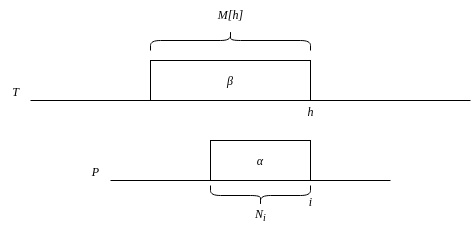
\includegraphics[width=.9\textwidth]{LaTeX/Figures/Zalg/Apostolicocase.png}
    \caption{One of the cases in the Apostolico-Giancarlo extension. The substring $\alpha$ in $P$ has length $N_i$ and $\beta$ in $T$ has length $M[h]$. When $M[h]>N_i$, then $\alpha$ matches $\beta$ but the next character is a mismatch. }
    \label{fig:Apostolicocase}
\end{figure}

The Apostolico-Giancarlo extension is detailed in algorithm \ref{alg:apostolicogiancarlo}. Gusfield\cite{Gusfield1997AlgorithmsOS} uses the concept of a "phase" and calls it the "phase algorithm", whereas here it is simply written as a loop for each alignment of $P$ with $T$. 

\begin{algorithm}[ht!]
\caption{The Apostolico-Giancarlo extension}\label{alg:apostolicogiancarlo}
\begin{algorithmic}
\State Preprocess the pattern just like the Boyer-Moore algorithm, yielding values for $L'(i)$, $l'(i)$, $R(x)$ and $N_i$. 
\State Align the left end of $P$ with the left end of $T$ and process $P$ from right-to-left. 
\State Let $j\leq m$ denote the position that the right end of $P$ is aligned with in $T$
\For{each alignment of $P$ with $T$}
    \State Let $i:=n$ and $h:=j$
    \State The following states the different cases depending on $M(h)$ and $N_i$
    \Loop\ Until $P$ is shifted. 
    \If{$M(h)$ is undefined or $M(h)=N_i=0$}
        \State Compare $T(h)$ with $P(i)$ and decrement $h$ and $i$ if they match. 
        \If{an occurrence of $P$ in $T$ is found or there is a mismatch}
        \State Set $M(j):=j-h$ with $j-h=n$ in the case of a match. 
        \State Shift as in Boyer-Moore. 
        \EndIf
    \ElsIf{$M(h)<N_i$ or $(M(h)=N_i$ and $0<N_i<i)$}
        \State The next $N_i$ characters are inferred to match. 
        \State Decrement both $i$ and $h$ by $M(h)$ and continue with the same alignment. 
    \ElsIf{$M(h)\geq N_i$ and $N_i=i>0$}
        \State The next $N_i$ characters match and $N_i=i$ so an occurrence has been found. 
        \State Set $M(j):=j-h$ and shift as in Boyer-Moore. 
    \ElsIf{$M(h)>N_i$ and $N_i<i$}
        \State The next $N_i$ characters match but $P(i-N_i)\neq T(h-N_i)$. 
        \State Set $M(j):=j-h$ 
        \State Shift as in Boyer-Moore based on a mismatch at position $i-N_i$. 
    \EndIf
    \EndLoop
\EndFor
\end{algorithmic}
\end{algorithm}

As explained, this extension ensures that a character in $T$ is involved in at most one match and one mismatch, using at most $2m$ comparisons which gives the $O(m)$ bound in all cases. 

